\documentclass[a4paper,12pt]{article}
\usepackage[utf8]{inputenc}
\usepackage[portuguese]{babel}
\usepackage{graphicx}
\usepackage{amsmath}
\usepackage{enumitem}
\usepackage{indentfirst}
\usepackage[colorlinks=true,linkcolor=black,urlcolor=black]{hyperref}
\usepackage{fancyhdr}
\usepackage{listings}
\usepackage{xcolor}
\usepackage{acronym}
\usepackage{dirtree}
\usepackage{adjustbox}
\usepackage{pdflscape}
\usepackage{float}
\usepackage{caption}
\usepackage{xurl}

\lstset{
    language=SQL,
    basicstyle=\ttfamily\small,
    keywordstyle=\color{blue},
    stringstyle=\color{red},
    commentstyle=\color{green!50!black},
    numberstyle=\tiny,
    numbers=left,
    stepnumber=1,
    numbersep=5pt,
    backgroundcolor=\color{gray!10},
    showspaces=false,
    showstringspaces=false,
    showtabs=false,
    tabsize=2,
    captionpos=b,
    breaklines=true,
    breakatwhitespace=true,
    breakautoindent=true,
    linewidth=\textwidth,
}

\pagestyle{fancy}
\fancyhf{}
\fancyfoot[R]{\thepage}
\renewcommand{\headrulewidth}{0pt}

\begin{document}

% Logo da universidade
\begin{figure}[H]
  \centering
  
\includegraphics[width=0.5\textwidth]{Anexos/UBI_LOGO.jpg}
\end{figure}

% Título e autor
\title{Projeto de Software Web, Móvel e na Nuvem\\Sistema de Gestão Digital para a Oficina Duarte \& Raposo}
\author{Tiago Dias Pereira - 55019}
\date{\today}

\maketitle
\newpage

% Sumário
\tableofcontents

\newpage

\section*{Resumo}
\addcontentsline{toc}{section}{Resumo}

Este relatório descreve o desenvolvimento integral de um sistema de gestão desenhado à medida para a oficina automóvel Duarte \& Raposo, no âmbito da unidade curricular de Projeto de Software Web, Móvel e na Nuvem. O objetivo prático é resolver um problema real com o qual lido diariamente no meu local de trabalho: a ineficiência operacional, a desorganização e a perda de histórico geradas pelo uso exclusivo de folhas de obra em papel.

O trabalho abrangeu todo o ciclo de vida do sistema: desde a engenharia de requisitos e modelação concetual, passando pela normalização do esquema lógico relacional (3FN) e implementação num SGBD SQL Server via Docker, até à construção de uma Aplicação Cliente (PWA e Dashboard) suportada por uma API em Node.js. A solução permite agora a gestão digital de veículos complexos (como autocaravanas), auditoria de colaboradores e processamento ágil para faturação.

\section*{Palavras-chave}
Informática Web; React; Node.js; SQL Server; PWA; Docker; Engenharia de Requisitos; Autocaravanas.

\newpage

\section{Introdução}
\subsection{Âmbito e Motivação}

No dia a dia da oficina Duarte \& Raposo, especializada em eletricidade, mecânica e autocaravanas, todo o processo de entrada de veículos e registo de peças é feito de forma manual. Este sistema baseado em papel tem várias falhas críticas: é difícil consultar o histórico de uma autocaravana que já lá esteve no ano passado, os papéis sujam-se ou perdem-se pela oficina, e no final da reparação perde-se muito tempo a fazer contas à mão para conseguir passar a fatura ao cliente.

A motivação para este projeto surge exatamente da vontade de juntar o útil ao agradável: aplicar os conhecimentos adquiridos ao longo do curso de Informática Web para desenvolver uma solução real que facilite não só o meu trabalho, mas o de toda a equipa. O foco vai estar especialmente nas autocaravanas, dado que são veículos complexos (com parte mecânica e parte habitacional) e exigem um registo mais detalhado que um veículo ligeiro comum.

\subsection{Objetivos da Implementação}
\begin{itemize}
    \item \textbf{Acabar com o papel:} Passar todo o registo de clientes, veículos e folhas de obra para uma base de dados digital e relacional, garantindo a integridade dos dados.
    \item \textbf{Aplicação Móvel (PWA):} Desenvolver uma interface em \textbf{React} leve e direta, para que qualquer mecânico consiga dar entrada a um carro no sistema usando o telemóvel, sem perder muito tempo.
    \item \textbf{Gestão no Computador:} Criar uma interface web \textit{desktop} (Dashboard) para o Duarte e o Raposo poderem ver o que está a ser feito, consultar históricos e ver as contas automáticas do IVA para a faturação.
    \item \textbf{Arquitetura e Portabilidade:} Construir o \textit{backend} em Node.js com base de dados \ac{SQL} Server, e utilizar o \textbf{Docker} para contentorizar o projeto. Isto vai garantir que o sistema corre sempre bem, quer esteja a programar no meu computador fixo ou num portátil novo, sem dores de cabeça com compatibilidades.
\end{itemize}

\clearpage

\section{Engenharia de Requisitos}

\subsection{Levantamento de Dados Físicos}
Como trabalho diretamente na oficina, o levantamento de requisitos foi muito direto e baseado na realidade operacional. Peguei nas folhas de obra e faturas em branco que usamos atualmente e retirei a informação essencial que tem de transitar para a plataforma digital:
\begin{itemize}
    \item \textbf{Dados do Cliente:} Nome, Morada, NIF e Telefone.
    \item \textbf{Dados do Veículo:} Matrícula, e, no caso das autocaravanas, a separação imperativa entre a Marca/Modelo do Chassis e a Marca da Célula.
    \item \textbf{Dados da Entrada:} Data, os quilómetros (KMS) com que o carro entrou, e espaço para observações gerais.
    \item \textbf{O Serviço:} As várias linhas de material gasto e horas de trabalho, com quantidade, preço unitário e categoria do serviço.
\end{itemize}

\subsection{Histórias de Utilizador (\textit{User Stories})}
Com base nas rotinas da equipa e nas dificuldades sentidas no "chão de oficina", estruturei as necessidades interativas do sistema:
\begin{itemize}
    \item \textit{"Como mecânico, preciso de abrir a app no telemóvel e registar a entrada de um carro em poucos cliques, para voltar rapidamente ao trabalho."}
    \item \textit{"Como mecânico, quero adicionar as peças e serviços que usei diretamente à folha de obra ativa daquele carro no exato momento em que as aplico."}
    \item \textit{"Como mecânico, preciso de uma secção de 'Conselhos' para avisar o cliente sobre peças que vão precisar de ser trocadas no futuro, para prestarmos um bom serviço preventivo."}
    \item \textit{"Como gestor, preciso que o sistema some os valores do material, faça o cálculo do IVA sozinho quando a reparação acaba, e identifique quem foi o mecânico responsável pela obra."}
\end{itemize}

\clearpage

\section{Modelação de Dados e Arquitetura}

\subsection{Modelo Relacional e Decisões de Desenho}
Para garantir a integridade referencial dos dados e mitigar as redundâncias presentes no modelo de papel (como escrever o nome do cliente dez vezes para o mesmo carro ao longo do ano), desenhei uma base de dados relacional (ver Anexos) que cumpre com os normativos da Terceira Forma Normal (3NF). 

Durante esta fase, tomei as seguintes opções técnicas para adaptar o sistema à realidade do negócio:

\begin{itemize}
    \item \textbf{Separação Estrutural das Autocaravanas:} Decidi modelar a entidade \textit{Autocaravana} separando explicitamente a parte mecânica (\texttt{Marca\_chassis}, \texttt{Modelo\_chassis}) da parte habitacional (\texttt{marca\_celula}). Isto é vital na nossa oficina, pois permite encomendar peças de motor à Fiat/Ford e peças de habitáculo a fornecedores de campismo de forma isolada e precisa.
    
    \item \textbf{Rastreabilidade Operacional (\textit{Auditing}):} No papel, as assinaturas perdem-se. Para resolver isto, criei a entidade \textit{Colaboradores}. Foi estabelecido um relacionamento onde cada \textit{Folha\_Obra} guarda obrigatoriamente a Chave Estrangeira do colaborador (\texttt{ID\_Colaborador}) que a registou, garantindo auditoria e responsabilização interna.
    
    \item \textbf{Preservação Fisco-Operacional (Soft Delete):} Numa empresa real, apagar dados com um \texttt{DELETE} pode destruir o histórico fiscal e garantias de peças. Para acautelar isto, implementei um sistema de \textit{Soft Delete}: adicionei o atributo \texttt{ativo} (booleano) às tabelas principais (Clientes, Veículos, Colaboradores). Os dados nunca são eliminados da base de dados, são apenas ocultados da interface.
\end{itemize}

O esquema relacional consolida-se assim em cinco entidades principais:
\begin{enumerate}
    \item \textbf{Colaboradores:} \underline{ID\_Colaborador}, Nome, Cargo, Email, Password\_Hash, Ativo.
    \item \textbf{Clientes:} \underline{ID\_Cliente}, Nome, Contribuinte\_NIF, Telefone, Morada, Ativo.
    \item \textbf{Autocaravanas:} \underline{Matricula}, Marca\_Chassis, Modelo\_Chassis, Marca\_Celula, Ano, Ativo, \textit{ID\_Cliente (FK)}.
    \item \textbf{Folhas\_Obra:} \underline{ID\_Folha}, Data\_Entrada, KMS\_Entrada, Estado\_Reparacao, Observacoes, Conselhos, \textit{Matricula (FK)}, \textit{ID\_Colaborador (FK)}.
    \item \textbf{Linhas\_Reparacao:} \underline{ID\_Linha}, Designacao, Quantidade, Valor\_Unitario, Categoria, \textit{ID\_Folha (FK)}.
\end{enumerate}

\subsection{A Escolha do Docker para Infraestrutura}
Em termos de arquitetura de servidor, decidi utilizar o \textbf{Docker} neste projeto, alinhando a solução com as melhores práticas de \textit{DevOps} lecionadas no curso. 

A vantagem principal para o meu caso de uso é a facilidade de criar ambientes isolados. Ao definir um ficheiro \texttt{docker-compose.yml}, consigo ter a base de dados SQL Server e, futuramente, a API em Node.js a correr em qualquer computador  através de um único comando. Isto evita que o meu computador fique "sujo" com serviços em segundo plano, consome menos recursos, e facilita drasticamente o \textit{deploy} do projeto para um servidor de produção quando a oficina adotar o sistema em definitivo.

\clearpage

% ==========================================
% SECÇÕES BASE PARA O FUTURO (A SUBSTITUIR DEPOIS)
% ==========================================

\section{Desenvolvimento da API REST (Backend)}

Esta secção documenta o estado atual da implementação do \textit{backend}, desenvolvido em Node.js. À data de escrita desta secção, encontram-se implementadas as três entidades independentes do modelo (Colaboradores, Clientes e Autocaravanas); as entidades relacionais mais complexas (Folhas de Obra e Linhas de Reparação) e a camada de interface (PWA e Dashboard) estão planeadas para a fase seguinte do projeto (ver secção~\ref{subsec:trabalho-futuro}).

\subsection{Arquitetura RESTful (Node.js)}
No desenvolvimento da camada de \textit{backend}, optou-se pela utilização do ambiente Node.js com a \textit{framework} Express. Esta API atua como o motor central de regras de negócio, comunicando diretamente com o SQL Server e expondo os \textit{endpoints} necessários para as operações \ac{CRUD}.

O código foi organizado de forma modular, separando claramente três responsabilidades:
\begin{itemize}
    \item \texttt{db.js} --- gestão centralizada da ligação à base de dados;
    \item \texttt{routes/} --- um ficheiro por entidade (\texttt{colaboradores.js}, \texttt{clientes.js}, \texttt{autocaravanas.js}), cada um definindo as suas próprias rotas através do \texttt{express.Router()};
    \item \texttt{server.js} --- ponto de entrada da aplicação, responsável apenas por montar as rotas e arrancar o servidor.
\end{itemize}

Esta separação, em vez de concentrar toda a lógica num único ficheiro, torna o código mais fácil de expandir à medida que novas entidades (como as Folhas de Obra) são adicionadas, e facilita a leitura do projeto em contexto de avaliação académica.

\subsection{Rotas Implementadas}
A Tabela~\ref{tab:rotas} resume os \textit{endpoints} atualmente disponíveis. Todas as entidades seguem o mesmo padrão \ac{CRUD}, com a particularidade de o método \texttt{DELETE} nunca remover fisicamente um registo (ver \textit{Soft Delete}, secção 3.1).

\begin{table}[H]
\centering
\begin{tabular}{|l|l|p{6.5cm}|}
\hline
\textbf{Método} & \textbf{Endpoint} & \textbf{Descrição} \\
\hline
GET & /api/colaboradores & Lista colaboradores ativos \\
GET & /api/colaboradores/:id & Obtém um colaborador \\
POST & /api/colaboradores & Cria colaborador (password encriptada com bcrypt) \\
PUT & /api/colaboradores/:id & Atualiza colaborador \\
DELETE & /api/colaboradores/:id & Desativa colaborador (soft delete) \\
\hline
GET & /api/clientes & Lista clientes ativos \\
GET & /api/clientes/:id & Obtém um cliente \\
POST & /api/clientes & Cria cliente \\
PUT & /api/clientes/:id & Atualiza cliente \\
DELETE & /api/clientes/:id & Desativa cliente (soft delete) \\
\hline
GET & /api/autocaravanas & Lista autocaravanas ativas (com nome do cliente) \\
GET & /api/autocaravanas/:matricula & Obtém uma autocaravana \\
POST & /api/autocaravanas & Cria autocaravana (valida existência do cliente) \\
PUT & /api/autocaravanas/:matricula & Atualiza autocaravana \\
DELETE & /api/autocaravanas/:matricula & Desativa autocaravana (soft delete) \\
\hline
\end{tabular}
\caption{Rotas da API implementadas até ao momento.}
\label{tab:rotas}
\end{table}

\subsection{Decisões Técnicas de Implementação}
\begin{itemize}
    \item \textbf{Pool de Ligações Único:} Em vez de abrir uma nova ligação ao SQL Server em cada pedido HTTP (\texttt{sql.connect()} por rota), foi implementado um pool de ligações único e partilhado por toda a aplicação (\texttt{db.js}), seguindo a recomendação da própria biblioteca \texttt{mssql}. Isto evita o esgotamento de ligações disponíveis sob carga.

    \item \textbf{Encriptação de \textit{Passwords}:} As \textit{passwords} dos colaboradores nunca são guardadas em texto simples. Antes de qualquer escrita na base de dados, são processadas com a biblioteca \texttt{bcrypt} (\textit{salt rounds} = 10), preparando o terreno para a futura implementação de autenticação (\textit{login}) na Fase 2.

    \item \textbf{Validação de Integridade Referencial ao Nível da Aplicação:} Antes de criar uma Autocaravana, a API confirma explicitamente que o \texttt{ID\_cliente} indicado existe e está ativo, devolvendo um erro \texttt{400} claro em caso negativo. Sem esta validação, um erro de chave estrangeira do SQL Server chegaria ao cliente da API de forma menos percetível.

    \item \textbf{Tratamento de Duplicados:} Os códigos de erro nativos do SQL Server para violação de restrições \texttt{UNIQUE} (2627/2601) são capturados e traduzidos para respostas HTTP \texttt{409 Conflict} com mensagens em português, em vez de expor o erro técnico da base de dados diretamente.
\end{itemize}

\subsection{Ambiente de Desenvolvimento Multiplataforma (Docker)}
Um aspeto prático relevante do desenvolvimento foi garantir que o ambiente Docker funciona de forma consistente em diferentes máquinas de desenvolvimento, nomeadamente entre um computador com processador Intel e um MacBook com Apple Silicon (M1/M2/M3/M4). A imagem oficial do SQL Server é distribuída apenas para arquitetura x86\_64, pelo que em Macs Apple Silicon a execução ocorre por emulação (Rosetta~2). Para tornar este comportamento explícito e evitar erros de arquitetura, foi adicionada a diretiva \texttt{platform: linux/amd64} ao serviço da base de dados no \texttt{docker-compose.yml}, garantindo o arranque correto do container independentemente do processador do anfitrião.

\subsection{Trabalho a Realizar}
\label{subsec:trabalho-futuro}
Ficam planeados para a fase seguinte do projeto:
\begin{itemize}
    \item Implementação das rotas de \textbf{Folhas de Obra} e \textbf{Linhas de Reparação}, que exigem lógica transacional (\texttt{sql.Transaction}) para garantir que a folha de obra e as suas linhas associadas são criadas de forma atómica;
    \item Implementação de \textbf{autenticação} (\textit{login} de colaboradores via \ac{JWT}, aproveitando o campo \texttt{Password\_Hash} já existente);
    \item Desenvolvimento da \textbf{PWA em React} para os mecânicos (visão mobile);
    \item Desenvolvimento do \textbf{Dashboard em React} para a gestão (visão desktop), incluindo o cálculo automático de IVA para faturação.
\end{itemize}

\section{Testes e Validação}

\subsection{Metodologia de Teste}
Os testes realizados até ao momento são testes manuais de integração, executados através da ferramenta \textit{Thunder Client}\footnote{Alternativamente, poderia ser usado o Postman; a escolha não afeta os resultados.} e da linha de comandos (\texttt{curl}), validando o comportamento de cada rota diretamente contra a base de dados SQL Server a correr em Docker. A automatização de testes (por exemplo, com \textit{Jest} e \textit{Supertest}) fica identificada como possível extensão para a fase seguinte.

\subsection{Casos de Teste Executados}
A Tabela~\ref{tab:testes} resume os cenários validados manualmente para as três entidades implementadas.

\begin{table}[H]
\centering
\begin{tabular}{|p{4.5cm}|p{7.5cm}|c|}
\hline
\textbf{Cenário} & \textbf{Resultado Esperado} & \textbf{OK?} \\
\hline
Criar cliente com todos os campos válidos & Resposta 201, registo devolvido com \texttt{ID\_cliente} & Sim \\
\hline
Listar clientes & Resposta 200, apenas clientes com \texttt{Ativo = 1} & Sim \\
\hline
Criar autocaravana com \texttt{id\_cliente} inexistente & Resposta 400, mensagem clara (sem expor erro SQL) & Sim \\
\hline
Criar autocaravana com matrícula já existente & Resposta 409 Conflict & Sim \\
\hline
Criar colaborador e confirmar que a \textit{password} não é devolvida em texto simples & Resposta 201, campo \texttt{password} ausente da resposta & Sim \\
\hline
Desativar (soft delete) um colaborador e tentar listá-lo & Não aparece na listagem, mas mantém-se na base de dados & Sim \\
\hline
\end{tabular}
\caption{Casos de teste manuais executados sobre a API.}
\label{tab:testes}
\end{table}

\subsection{Validação de Integridade Referencial}
Foram realizadas tentativas propositadas de inserção de dados inconsistentes para confirmar que o sistema bloqueia operações ilícitas --- por exemplo, associar uma autocaravana a um \texttt{ID\_cliente} inexistente ou já inativo. Estas validações são feitas explicitamente ao nível da aplicação (e não apenas por rejeição da base de dados), permitindo devolver mensagens de erro percetíveis ao utilizador final da API.

\textit{[Nota de Edição: inserir aqui as capturas de ecrã do Thunder Client/Postman correspondentes aos testes da Tabela~\ref{tab:testes}, uma por cada pedido relevante, por exemplo:]}
% \begin{figure}[H]
%   \centering
%   \includegraphics[width=0.9\textwidth]{Anexos/teste_post_cliente.png}
%   \caption{Criação de um cliente via POST /api/clientes.}
% \end{figure}

\section{Conclusão}

\textit{[Nota de Edição: esta é uma síntese do estado intercalar do projeto; será revista e completada no relatório final, após a conclusão das Folhas de Obra, autenticação e interfaces React.]}

O desenvolvimento deste projeto, até ao momento, percorreu com sucesso as fases de levantamento de requisitos, modelação de dados e implementação inicial do \textit{backend}, tendo o modelo relacional e a infraestrutura Docker sido validados na prática.

\textbf{O que foi conseguido até ao momento:}
Foi desenhado e fundamentado um modelo de dados relacional adaptado à realidade oficinal, com foco nas autocaravanas, e implementado o \textit{backend} correspondente às três entidades independentes do modelo (Colaboradores, Clientes e Autocaravanas), com \ac{CRUD} completo, validações de integridade referencial e testes manuais documentados na secção anterior. A arquitetura \textit{containerizada} em Docker provou ser eficaz e portátil entre diferentes máquinas de desenvolvimento.

\textbf{O que falta concluir:} as rotas de Folhas de Obra e Linhas de Reparação (com lógica transacional), a autenticação de colaboradores, e a camada de interface --- a PWA em React para os mecânicos e o Dashboard para a gestão, incluindo o cálculo automático de IVA para faturação.

De uma forma geral, os objetivos propostos na fase de idealização estão a ser cumpridos progressivamente, com o backend a substituir já parte do fluxo em papel. A conclusão integral do sistema, com a camada de interface funcional, permitirá validar por completo a solução junto da oficina Duarte \& Raposo.

\clearpage

\section{Referências Bibliográficas}

\begin{itemize}
    \item Documentação Oficial Docker. \textit{Docker Compose Overview}. Disponível em: \url{https://docs.docker.com/compose/}
    \item Documentação Microsoft. \textit{SQL Server on Linux}. Disponível em: \url{https://learn.microsoft.com/en-us/sql/linux/}
    \item MDN Web Docs. \textit{Progressive Web Apps (PWAs)}. Disponível em: \url{https://developer.mozilla.org/en-US/docs/Web/Progressive_web_apps}
\end{itemize}

\section*{Acrónimos}
\addcontentsline{toc}{section}{Acrónimos}
\begin{acronym}[UBI]
    \acro{UBI}{Universidade da Beira Interior}
    \acro{API}{Application Programming Interface}
    \acro{SQL}{Structured Query Language}
    \acro{PWA}{Progressive Web App}
    \acro{CRUD}{Create, Read, Update, Delete}
    \acro{SGBD}{Sistema de Gestão de Bases de Dados}
    \acro{3FN}{Terceira Forma Normal}
    \acro{JWT}{JSON Web Token}
\end{acronym}

\clearpage

% --- ANEXOS ---
\section{Anexos}
\addcontentsline{toc}{section}{Anexos}

\subsection*{Anexo I: Diagrama da Base de Dados}
 \begin{figure}[H]
    \centering
    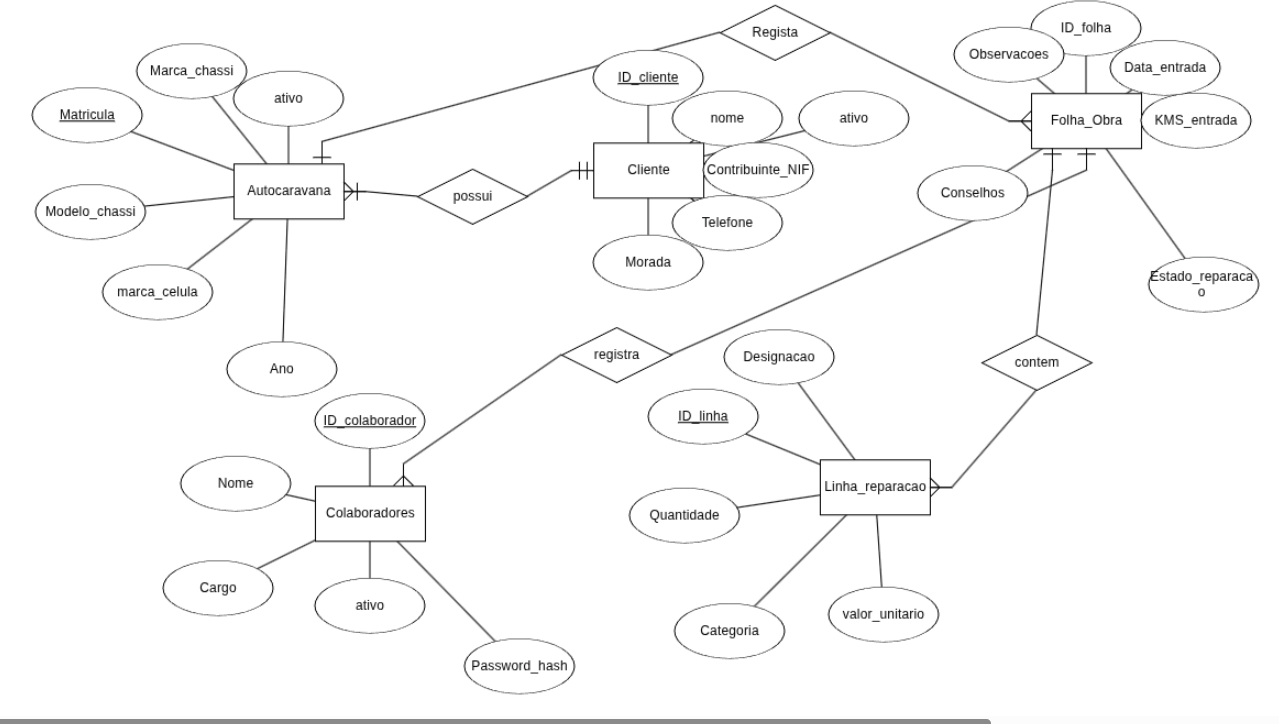
\includegraphics[width=0.9\textwidth]{Anexos/Diagrama.png}
    \caption{Diagrama concetual gerado no ERDPlus.}
 \end{figure}

\subsection*{Anexo II: Esquema Relacional da Base de Dados}
 \begin{figure}[H]
    \centering
    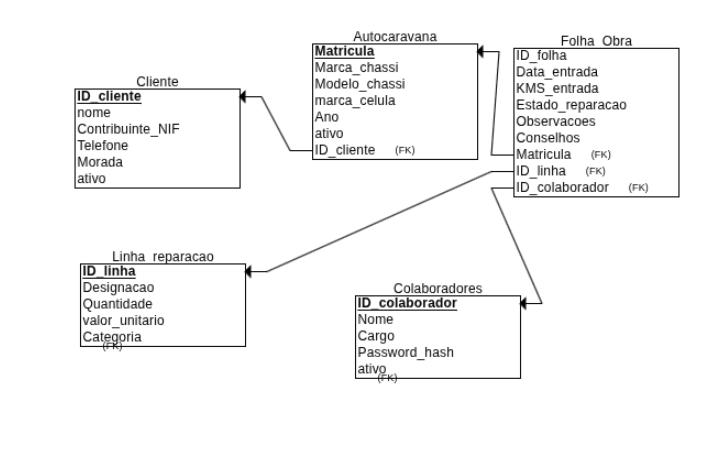
\includegraphics[width=0.9\textwidth]{Anexos/Esquema_relacional.png}
    \caption{Esquema Relacional final gerado no ERDPlus.}
 \end{figure}

\end{document}